\section{Conclusiones}

\subsection{Comparación de tiempos}

En esta sección presentaremos una comparativa entre los tiempos que tarda cada algoritmo a medida que aumenta el tamaño de la imagen. Para tal fin testamos cada algoritmo con imágenes cuadradas generadas aleatoriamente que van aumentando su tamaño, y creemos que es una forma correcta de comparar los tiempos ya que la complejidad de cada algoritmo es mas independiente de la información que tenga la imagen que del tamaño debido a que las iteraciones depende directamente de este.

\begin{figure}[h]
       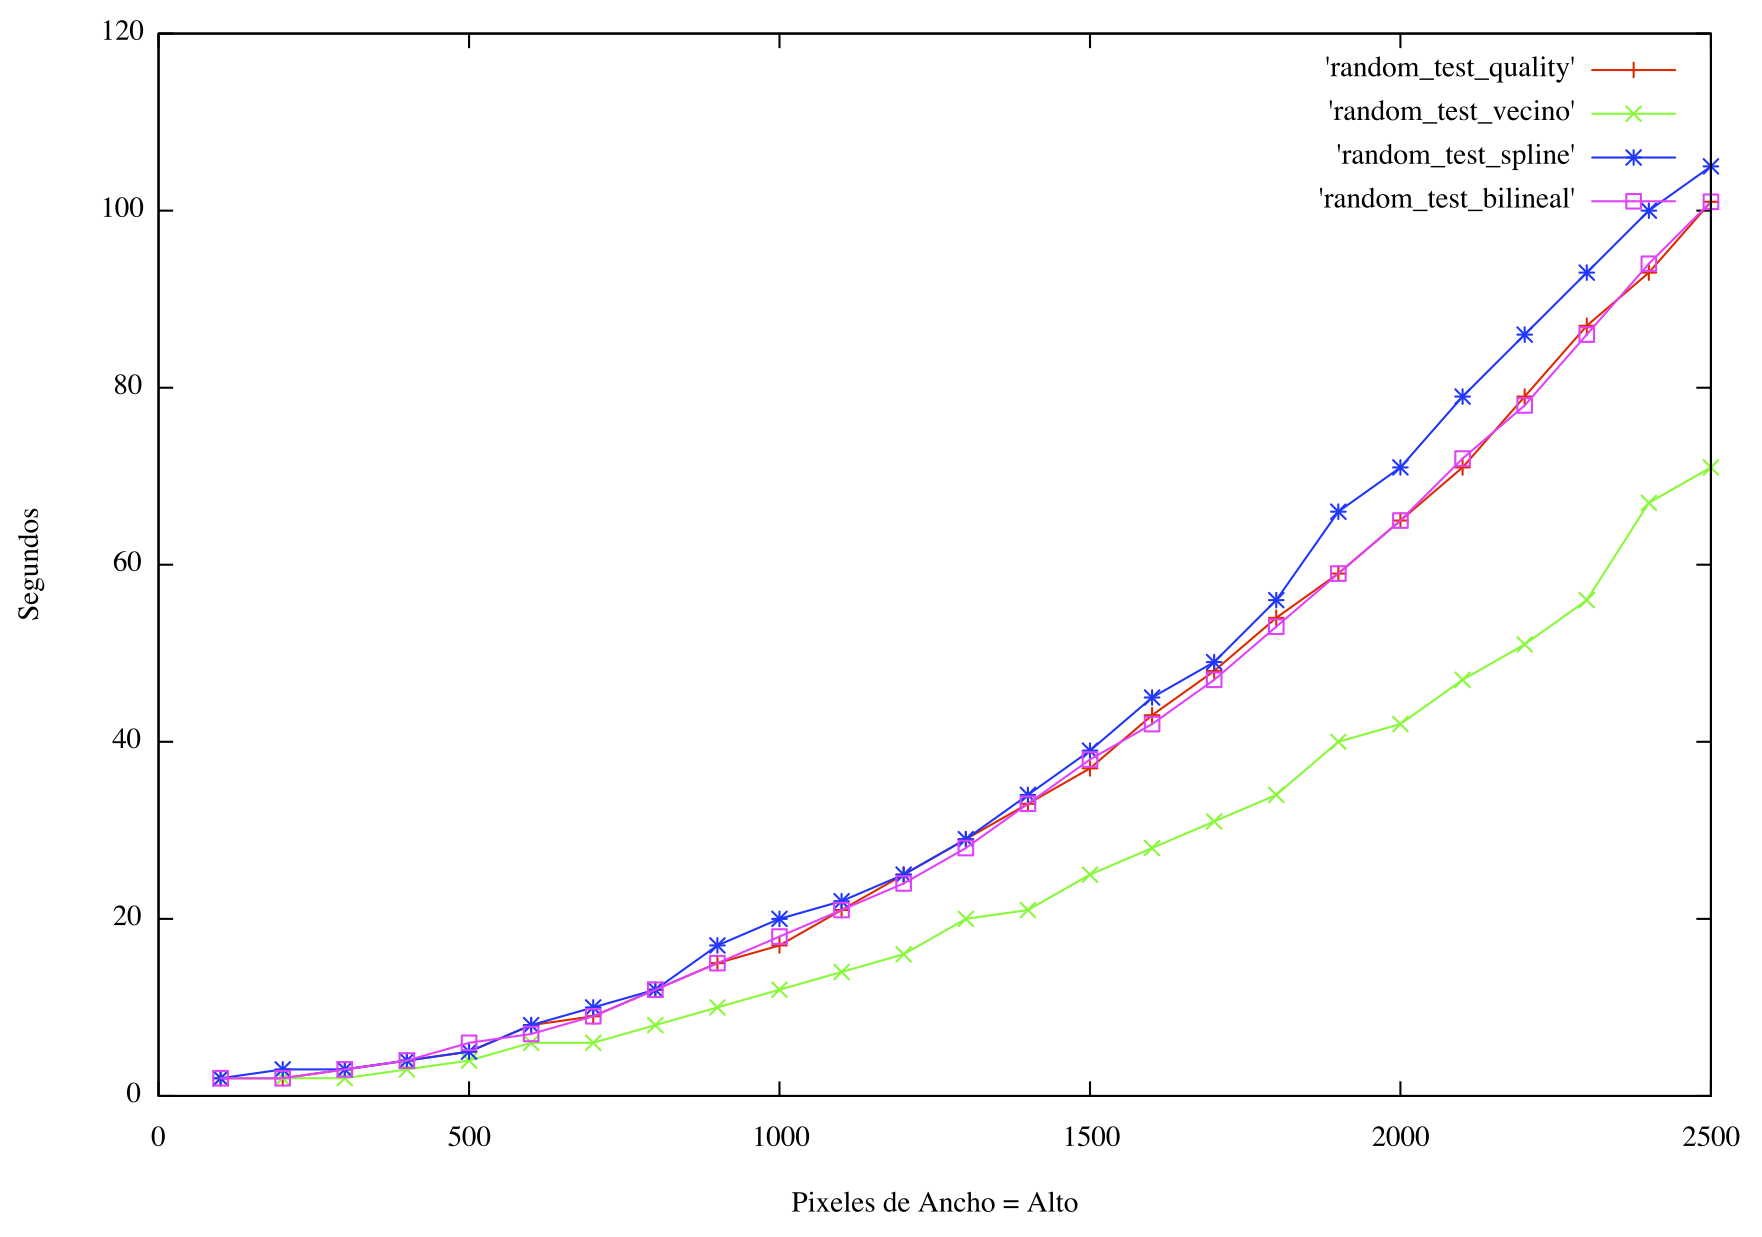
\includegraphics[width=1\textwidth]{imagenes/tiempo_algoritmos_random.png}
\end{figure}

Vecinos al ser el más simple, tiene sentido que haya tardado menos. Lo único que hace es recorrer la imagen y rellenar por cada color faltante de cada pixel, de, valga la redundancia, sus vecinos que captaron ese color en la bayerización. Bilineal en segundo puesto, ya que realiza un promedio y necesita ver más puntos. \\
Tanto Direccional y Quality, utilizan bilineal ya que no son algoritmos de aproximación de cero, si no de mejora. Por lo que ya tienen una cota inferior. Igualmente es notable que Quality siendo el mejor resultado, como venimos viendo en puntos anteriores y un detalle mejor en la próxima sección, también sea el de menor tiempo. Esto se debe a que tiene una cuenta parecida al bilineal pero en pocos píxeles, a diferencia de Direccional que resuelve un sistema de ecuaciones por cada fila y columna.\\
Igualmente no es poco notar que son bastantes lentos los algoritmos, y las pruebas si bien fueron con imágenes relativamente grandes, no alcanzan a las cámaras promedio que claramente no tardan 10 segundos en resolver la foto final. O existen optimizaciones que no llegamos a hacer o hay un mejor aprovechamiento del hardware, paralelismo, etc.
Como el algoritmo de HighQuality solamente procesa los verdes de la imagen, requerira un $"$poco$"$ más de tiempo para imagenes que tengan una mayor calidad para ese color.




\subsection{Comparación de calidad}
En esta sección compararemos solo los verdes de las imágenes y veremos los resultados utilizando PSNR. Recordemos que este término, calcula nivel de ruido en una señal.

\begin{figure}[h]
       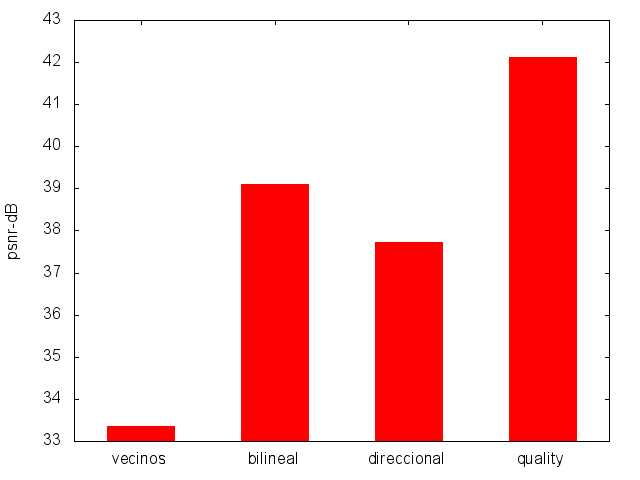
\includegraphics[scale=0.8]{imagenes/quality_performance.png}
       \caption{Img1}
\end{figure}

Como venimos viendo en otros ejemplos, img9, img12, y este, como era esperado, el vecinos es el que peor hizo, y quality fue el mejor. Sin embargo notemos que Spline si bien 
tendría que tener un valor mayor que bilineal ya que subjetivamente notamos mejora entre ellos, no lo tiene, es 
decir, el nivel de ruido es mayor en el direccional. Esto tiene sentido en la medida que el algoritmo direccional 
utiliza toda la fila y toda la columna para calcular el valor de las coordenadas $b_j$, $c_j$ y $d_j$ por lo que está 
sujeto a valores distintos al valor final, a diferencia de Bilineal que está sujeto a sus vecinos directos que es 
mucho más probable que tengan un valor más próximo. 


\subsection{Algoritmos}
En base a los algoritmos presentados, concluimos que a partir del tiempo de cómputo y resultados que ofrecen los mismos, siempre conviene optar por el algoritmo de HighQuality, ya que como se observa en las secciones anteriores, la calidad que ofrece es extremadamente buena y el tiempo que tarda es aceptable.
Otra cosa que nos llamo la atención fueron los resultados obtenidos por las dos interpolaciones bilineales y direccionales, ya que si bien en teoría la direccional debería obtener mejores resultados, estos solo se aprecian al mirarlos, es decir subjetivamente, ya que objetivamente el bilineal aproxima mejor los colores originales y obtiene un menor ruido en la señal del color verde.

\subsection{Bordes}
En caso de una imagen con cambios grandes en zonas pequeñas, todos los algoritmos tienden a fallar en esas zonas.
Esto se debe a que todos los algoritmos dependen fuertemente de los pixeles próximos cercanos, los cuales poseen valores muy distintos al valor a calcular. Esto es denominado borde.

Otro punto interesante es que si bien el algoritmo de High Quality funcionó mejor objetiva y subjetivamente para las imagenes que son fotografiías esto no fué así en el caso de la imagen $"$colores$"$. Pensamos que esto se debe a que este procedimiento fué especialmente pensado para fotografías, es decir imagenes con bordes mas suaves o sin tanta saturación de color de cada lado del borde. Y que es por esto que en este caso los resultados dieron casi lo contrario de todo el resto (vecinos fué el mejor en todo sentido).

\subsection{Otro uso}
Si bien el TP está apuntado a los algoritmos que corren en las cámaras de fotos, un uso útil puede ser el de compresión de imágenes, ya que bayerizando la imagen original reduce en un tercio su tamaño y en poco tiempo (menor aún en la práctica cuando lo usan las camáras digitales) se puede obtener la original, o al menos una aproximación bastante acertada de la misma.